%============================================================
%  Data Center Availability: Methodology & Topology Comparison
%  Beamer (metropolis) — full technical deck
%  Compile: pdflatex data_center_availability.tex  (x2)
%           (lualatex/xelatex give the Fira font; pdflatex falls back)
%============================================================
\documentclass[aspectratio=169,10pt]{beamer}

\usetheme{metropolis}
\metroset{block=fill}

\usepackage{booktabs}
\usepackage{colortbl}
\usepackage{amsmath}
\usepackage{tikz}
\usepackage{pgfplots}
\pgfplotsset{compat=1.18}
\usetikzlibrary{positioning,calc,arrows.meta,fit,backgrounds}

%---- Palette ------------------------------------------------
\definecolor{accent}{HTML}{1F6FB2}   % blue  = redundant / result
\definecolor{surf}{HTML}{F2F4F7}     % light surface
\definecolor{surf2}{HTML}{E1ECF4}    % accent surface
\definecolor{edge}{HTML}{8A94A6}     % connectors

\setbeamercolor{frametitle}{bg=accent}

%---- RBD node styles ---------------------------------------
\tikzset{
  box/.style   ={draw=edge, rounded corners=3pt, minimum width=2.6cm,
                 minimum height=1.05cm, align=center, font=\scriptsize,
                 fill=surf, thick},
  % redundant stage: double border in accent
  redbox/.style={box, draw=accent, double, double distance=1.3pt, line width=0.7pt},
  load/.style  ={draw=accent, line width=1.4pt, rounded corners=3pt,
                 minimum width=2.4cm, minimum height=1.25cm, align=center,
                 font=\scriptsize\bfseries, fill=surf2},
  cont/.style  ={box, minimum width=6.2cm, minimum height=0.95cm},
  redcont/.style={cont, draw=accent, double, double distance=1.3pt, line width=0.7pt},
  flow/.style  ={-{Latex[length=2mm]}, edge, thick},
  tag/.style   ={font=\tiny\bfseries, text=accent},
}

\title{Data Center Availability}
\subtitle{Calculation Methodology \& Topology Comparison (Tier I--IV)}
\author{American Terawatt}
\date{\today}

\begin{document}

\maketitle

\begin{frame}{Agenda}
  \tableofcontents
\end{frame}

%============================================================
\section{Methodology}
%============================================================

\begin{frame}{What ``availability'' means}
  Availability is the fraction of time a facility (or system) can deliver IT load
  without interruption, measured over a defined period (typically a rolling 12 months).

  \vspace{0.6em}
  \begin{block}{Core relationship}
    \[
      A \;=\; \frac{\text{Uptime}}{\text{Uptime}+\text{Downtime}}
        \;=\; \frac{\mathrm{MTBF}}{\mathrm{MTBF}+\mathrm{MTTR}}
    \]
  \end{block}

  \vspace{0.3em}
  where \textbf{MTBF} is mean time between failures and \textbf{MTTR} is mean time to
  repair/recover. Reported as a percentage or in ``nines.''
\end{frame}

\begin{frame}{The language of nines}
  \centering
  \renewcommand{\arraystretch}{1.25}
  \begin{tabular}{lcc}
    \toprule
    \textbf{Availability} & \textbf{Nines} & \textbf{Allowable downtime / yr} \\
    \midrule
    99\,\%      & two   & $\approx$ 3.65 days   \\
    99.9\,\%    & three & $\approx$ 8.77 hours  \\
    99.99\,\%   & four  & $\approx$ 52.6 minutes\\
    99.999\,\%  & five  & $\approx$ 5.26 minutes\\
    99.9999\,\% & six   & $\approx$ 31.5 seconds\\
    \bottomrule
  \end{tabular}

  \vspace{1em}
  \small Every additional nine cuts allowable downtime by a factor of ten.
\end{frame}

\begin{frame}{Combining components}
  A facility is modeled as a reliability block diagram (RBD) of components in
  \emph{series} and \emph{parallel}.

  \vspace{0.4em}
  \begin{columns}[T]
    \column{0.5\textwidth}
      \begin{block}{Series — all required}
        \[ A = \prod_i A_i \]
        Any element fails $\Rightarrow$ outage. Always \emph{below} the weakest link.
      \end{block}
    \column{0.5\textwidth}
      \begin{block}{Parallel — redundant}
        \[ A = 1 - \prod_i (1-A_i) \]
        Survives if $\geq 1$ path works. Redundancy raises $A$ sharply.
      \end{block}
  \end{columns}

  \vspace{0.5em}
  \begin{alertblock}{$N{+}1$ unit group (tolerates one failure)}
    \[ A_{\text{grp}} = A^{N+1} + (N{+}1)\,A^{N}(1-A) \]
  \end{alertblock}
\end{frame}

\begin{frame}{Modeling assumptions}
  \begin{columns}[T]
    \column{0.52\textwidth}
      \textbf{Per-unit availabilities} (illustrative, single-unit MTBF/MTTR)
      \vspace{0.3em}
      \footnotesize
      \renewcommand{\arraystretch}{1.15}
      \begin{tabular}{lc}
        \toprule
        Component & $A_{\text{unit}}$ \\
        \midrule
        Utility feed      & 0.99900 \\
        Generator         & 0.99500 \\
        UPS module        & 0.99950 \\
        MV switchgear     & 0.99999 \\
        LV switchgear     & 0.99998 \\
        PDU               & 0.99995 \\
        Busway            & 0.99999 \\
        Chiller           & 0.99500 \\
        Pump              & 0.99900 \\
        CRAH unit         & 0.99900 \\
        \bottomrule
      \end{tabular}
    \column{0.48\textwidth}
      \textbf{Frameworks}
      \begin{itemize}
        \item Uptime Institute Tier standard (I--IV)
        \item TIA-942 infrastructure standard
        \item RBD, FMEA, Monte Carlo for complex topologies
      \end{itemize}
      \vspace{0.6em}
      \textbf{Scope}
      \begin{itemize}
        \item Facility \emph{infrastructure} availability
        \item Planned maintenance excluded (concurrently maintainable)
        \item Facility $=$ Power path $\times$ Cooling path
      \end{itemize}
  \end{columns}
\end{frame}

%============================================================
\section{Tier I \& II (baseline)}
%============================================================

\begin{frame}{Tier I topology --- $N$, single path (reference)}
  \centering
  \resizebox{0.94\textwidth}{!}{%
  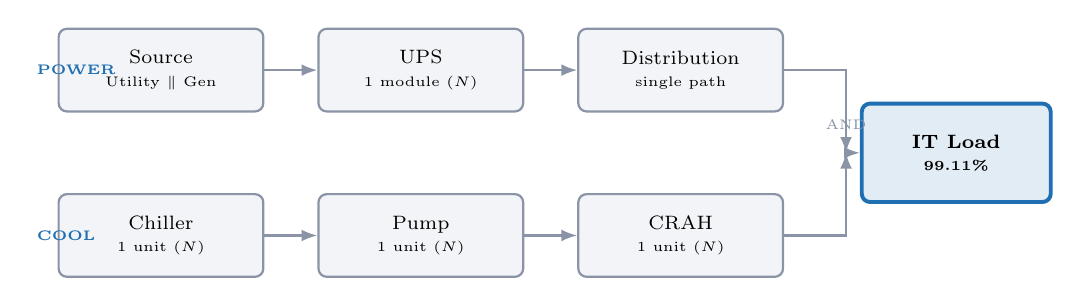
\begin{tikzpicture}
    \node[box] (S) at (0,2.1)  {Source\\{\tiny Utility $\parallel$ Gen}};
    \node[box] (U) at (3.3,2.1){UPS\\{\tiny 1 module ($N$)}};
    \node[box] (D) at (6.6,2.1){Distribution\\{\tiny single path}};
    \node[box] (C) at (0,0)   {Chiller\\{\tiny 1 unit ($N$)}};
    \node[box] (P) at (3.3,0) {Pump\\{\tiny 1 unit ($N$)}};
    \node[box] (R) at (6.6,0) {CRAH\\{\tiny 1 unit ($N$)}};
    \node[load] (L) at (10.1,1.05){IT Load\\{\tiny 99.11\%}};
    \draw[flow] (S) -- (U);   \draw[flow] (U) -- (D);
    \draw[flow] (C) -- (P);   \draw[flow] (P) -- (R);
    \draw[flow] (D.east) -| (8.7,1.05);
    \draw[flow] (R.east) -| (8.7,1.05);
    \draw[flow] (8.7,1.05) -- (L.west);
    \node[font=\tiny, text=edge] at (8.7,1.4) {AND};
    \node[tag, anchor=west] at (-1.7,2.1) {POWER};
    \node[tag, anchor=west] at (-1.7,0)   {COOL};
  \end{tikzpicture}}

  \vspace{0.5em}
  {\footnotesize No redundancy anywhere; single distribution path. \emph{Not} concurrently maintainable ---
   planned maintenance requires a shutdown. Model $\approx$ 99.11\,\% ($\approx$78 h/yr);
   Uptime Institute reference 99.671\,\% ($\approx$28.8 h/yr).}
\end{frame}

\begin{frame}{Tier II topology --- $N{+}1$ components, single path (reference)}
  \centering
  \resizebox{0.94\textwidth}{!}{%
  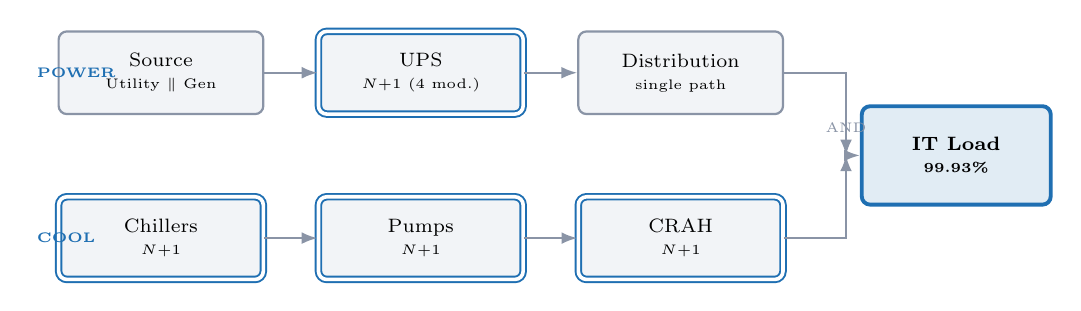
\begin{tikzpicture}
    \node[box]    (S) at (0,2.1)  {Source\\{\tiny Utility $\parallel$ Gen}};
    \node[redbox] (U) at (3.3,2.1){UPS\\{\tiny $N{+}1$ (4 mod.)}};
    \node[box]    (D) at (6.6,2.1){Distribution\\{\tiny single path}};
    \node[redbox] (C) at (0,0)   {Chillers\\{\tiny $N{+}1$}};
    \node[redbox] (P) at (3.3,0) {Pumps\\{\tiny $N{+}1$}};
    \node[redbox] (R) at (6.6,0) {CRAH\\{\tiny $N{+}1$}};
    \node[load] (L) at (10.1,1.05){IT Load\\{\tiny 99.93\%}};
    \draw[flow] (S) -- (U);   \draw[flow] (U) -- (D);
    \draw[flow] (C) -- (P);   \draw[flow] (P) -- (R);
    \draw[flow] (D.east) -| (8.7,1.05);
    \draw[flow] (R.east) -| (8.7,1.05);
    \draw[flow] (8.7,1.05) -- (L.west);
    \node[font=\tiny, text=edge] at (8.7,1.4) {AND};
    \node[tag, anchor=west] at (-1.7,2.1) {POWER};
    \node[tag, anchor=west] at (-1.7,0)   {COOL};
  \end{tikzpicture}}

  \vspace{0.5em}
  {\footnotesize Redundant capacity components ($N{+}1$) but a single, non-redundant distribution path
   $\Rightarrow$ \emph{not} concurrently maintainable. Same component RBD as Tier III;
   the difference is planned-maintenance downtime. Model $\approx$ 99.93\,\% ($\approx$6.3 h/yr);
   Uptime Institute reference 99.741\,\% ($\approx$22 h/yr).}
\end{frame}

%============================================================
\section{Tier III (N+1)}
%============================================================

\begin{frame}{Tier III topology --- $N{+}1$, concurrently maintainable}
  \centering
  \resizebox{0.98\textwidth}{!}{%
  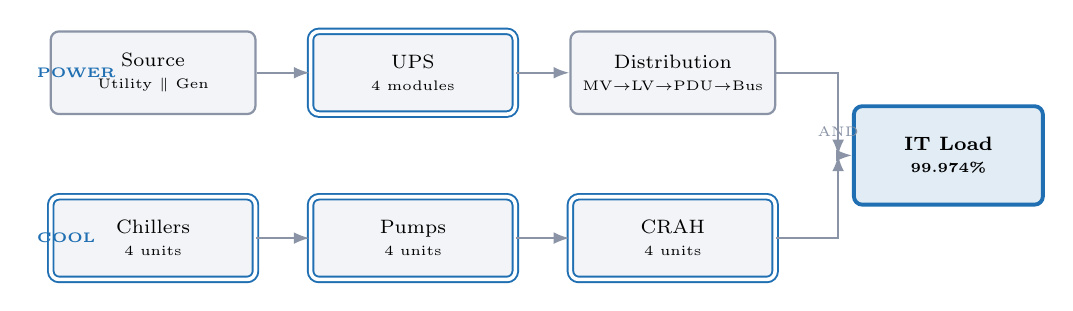
\begin{tikzpicture}
    % power row
    \node[box]    (S) at (0,2.1)  {Source\\{\tiny Utility $\parallel$ Gen}};
    \node[redbox] (U) at (3.3,2.1){UPS\\{\tiny 4 modules}};
    \node[box]    (D) at (6.6,2.1){Distribution\\{\tiny MV$\to$LV$\to$PDU$\to$Bus}};
    % cooling row
    \node[redbox] (C) at (0,0)   {Chillers\\{\tiny 4 units}};
    \node[redbox] (P) at (3.3,0) {Pumps\\{\tiny 4 units}};
    \node[redbox] (R) at (6.6,0) {CRAH\\{\tiny 4 units}};
    % load
    \node[load]   (L) at (10.1,1.05){IT Load\\{\tiny 99.974\%}};
    % flows
    \draw[flow] (S) -- (U);   \draw[flow] (U) -- (D);
    \draw[flow] (C) -- (P);   \draw[flow] (P) -- (R);
    \draw[flow] (D.east) -| (8.7,1.05);
    \draw[flow] (R.east) -| (8.7,1.05);
    \draw[flow] (8.7,1.05) -- (L.west);
    \node[font=\tiny, text=edge] at (8.7,1.35) {AND};
    % row labels
    \node[tag, anchor=west] at (-1.6,2.1) {POWER};
    \node[tag, anchor=west] at (-1.6,0)   {COOL};
  \end{tikzpicture}}

  \vspace{0.5em}
  {\footnotesize
   \textcolor{accent}{\rule{0.55em}{0.55em}} double border $=N{+}1$ redundant stage
   \quad$\bullet$\quad single border $=$ single (concurrently maintainable) path.}
\end{frame}

\begin{frame}{Tier III results}
  \centering
  \renewcommand{\arraystretch}{1.2}
  \begin{tabular}{lcc}
    \toprule
    \textbf{Stage} & \textbf{Availability} & \textbf{Downtime / yr} \\
    \midrule
    Source (Utility $\parallel$ Gen) & 99.9995\,\% & 2.6 min \\
    UPS ($N{+}1$)                    & 99.9998\,\% & 0.8 min \\
    Distribution (series)            & 99.9910\,\% & 47 min  \\
    \addlinespace
    \textbf{Power path}              & \textbf{99.9904\,\%} & \textbf{51 min} \\
    \midrule
    Chillers ($N{+}1$)               & 99.9851\,\% & 78 min \\
    Pumps ($N{+}1$)                  & 99.9994\,\% & 3 min  \\
    CRAH ($N{+}1$)                   & 99.9994\,\% & 3 min  \\
    \addlinespace
    \textbf{Cooling path}            & \textbf{99.9839\,\%} & \textbf{85 min} \\
    \midrule
    \rowcolor{surf2}
    \textbf{Facility} $=$ Power $\times$ Cooling & \textbf{99.974\,\%} & \textbf{$\approx$ 135 min (2.26 h)} \\
    \bottomrule
  \end{tabular}

  \vspace{0.8em}
  \small The single distribution path is the weakest link, capping the power path at $\approx$ four nines.
\end{frame}

%============================================================
\section{Tier IV (2N)}
%============================================================

\begin{frame}{Tier IV topology --- $2N$, fault tolerant}
  \centering
  \resizebox{0.98\textwidth}{!}{%
  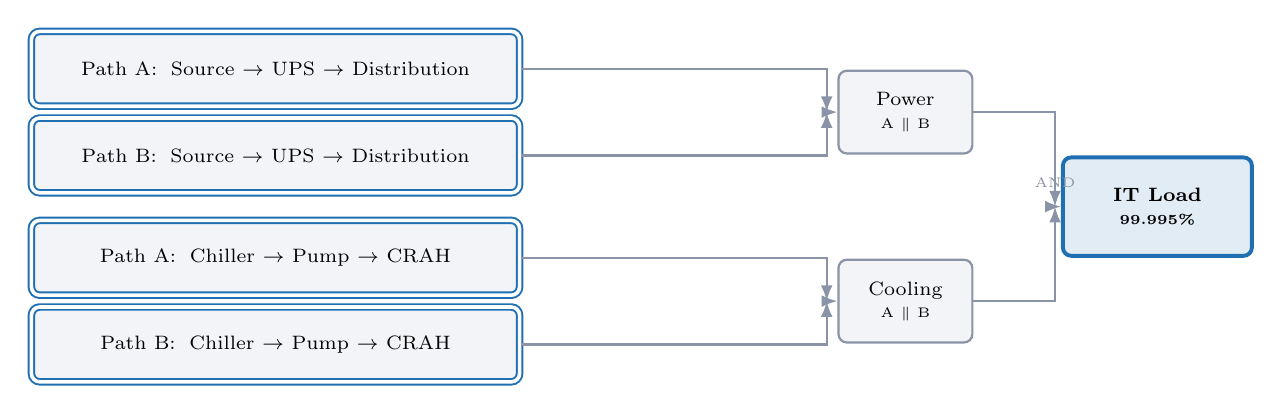
\begin{tikzpicture}
    % power 2N
    \node[redcont] (PA) at (0,2.7) {Path A:\; Source $\to$ UPS $\to$ Distribution};
    \node[redcont] (PB) at (0,1.6) {Path B:\; Source $\to$ UPS $\to$ Distribution};
    \node[box, minimum width=1.7cm] (PW) at (8.0,2.15) {Power\\{\tiny A $\parallel$ B}};
    \draw[flow] (PA.east) -| (7.0,2.15);
    \draw[flow] (PB.east) -| (7.0,2.15);
    \draw[flow] (7.0,2.15) -- (PW.west);
    % cooling 2N
    \node[redcont] (CA) at (0,0.3)  {Path A:\; Chiller $\to$ Pump $\to$ CRAH};
    \node[redcont] (CB) at (0,-0.8) {Path B:\; Chiller $\to$ Pump $\to$ CRAH};
    \node[box, minimum width=1.7cm] (CW) at (8.0,-0.25) {Cooling\\{\tiny A $\parallel$ B}};
    \draw[flow] (CA.east) -| (7.0,-0.25);
    \draw[flow] (CB.east) -| (7.0,-0.25);
    \draw[flow] (7.0,-0.25) -- (CW.west);
    % converge to load
    \node[load] (L) at (11.2,0.95) {IT Load\\{\tiny 99.995\%}};
    \draw[flow] (PW.east) -| (9.9,0.95);
    \draw[flow] (CW.east) -| (9.9,0.95);
    \draw[flow] (9.9,0.95) -- (L.west);
    \node[font=\tiny, text=edge] at (9.9,1.25) {AND};
  \end{tikzpicture}}

  \vspace{0.5em}
  {\footnotesize Every stage duplicated end-to-end (\textcolor{accent}{$2N$}) --- no single non-redundant link;
   unavailable only if \emph{both} A and B fail.}
\end{frame}

\begin{frame}{Tier IV results}
  \centering
  \renewcommand{\arraystretch}{1.25}
  \begin{tabular}{lcc}
    \toprule
    \textbf{Subsystem} & \textbf{Availability} & \textbf{Downtime / yr} \\
    \midrule
    Power --- per side (series string) & 99.8905\,\% & --- \\
    \rowcolor{surf}
    Power --- $2N$ ($A \parallel B$)   & 99.99988\,\% & $<$ 1 min \\
    \addlinespace
    Cooling --- per side (series string) & 99.3011\,\% & --- \\
    \rowcolor{surf}
    Cooling --- $2N$ ($A \parallel B$) & 99.99512\,\% & 26 min \\
    \midrule
    \rowcolor{surf2}
    \textbf{Facility} $=$ Power $\times$ Cooling & \textbf{99.995\,\%} & \textbf{$\approx$ 26 min} \\
    \bottomrule
  \end{tabular}

  \vspace{0.8em}
  \small Paralleling two full paths, $A = 1-(1-A_{\text{path}})^2$, \emph{squares} each side's
  unavailability. Cooling is now the limiting path (single-side chillers are the weakest string).
\end{frame}

%============================================================
\section{Comparison \& Conclusions}
%============================================================

\begin{frame}{Four-tier reference}
  \centering
  \renewcommand{\arraystretch}{1.3}
  \footnotesize
  \begin{tabular}{lcccc}
    \toprule
    & \textbf{Redundancy} & \textbf{Conc.\ maint.} & \textbf{Model $A$ (downtime)} & \textbf{Uptime ref.} \\
    \midrule
    Tier I   & $N$, single path          & no  & 99.11\,\% ($\approx$78 h)    & 99.671\,\% (28.8 h) \\
    Tier II  & $N{+}1$ comp., single path & no  & 99.93\,\% ($\approx$6.3 h)   & 99.741\,\% (22 h)   \\
    Tier III & $N{+}1$, redundant path    & yes & 99.974\,\% ($\approx$135 min)& 99.982\,\% (1.6 h)  \\
    \rowcolor{surf2}
    Tier IV  & $2N$, fault tolerant       & yes & 99.995\,\% ($\approx$26 min) & 99.995\,\% (26.3 min) \\
    \bottomrule
  \end{tabular}

  \vspace{0.8em}
  \begin{columns}[T]
    \column{0.5\textwidth}
      \textbf{Model} --- our per-unit component RBD. Tiers I--II add assumed
      planned-maintenance shutdowns (12 h / 4 h); III--IV exclude planned work.
    \column{0.5\textwidth}
      \textbf{Uptime ref.} --- Uptime Institute's widely-cited legacy figures.
      They are design classifications, not measured values; the Institute has since
      de-emphasised specific percentages.
  \end{columns}
\end{frame}

\begin{frame}{Tier III vs.\ Tier IV}
  \begin{columns}[c]
    \column{0.52\textwidth}
      \renewcommand{\arraystretch}{1.3}
      \footnotesize
      \begin{tabular}{lcc}
        \toprule
         & \textbf{Tier III} & \textbf{Tier IV} \\
         & ($N{+}1$) & ($2N$) \\
        \midrule
        Redundancy   & unit-level & full path \\
        Distribution & single path & dual A/B \\
        Fault tolerant & no & yes \\
        Availability & 99.974\,\% & 99.995\,\% \\
        Downtime/yr  & $\approx$135 min & $\approx$26 min \\
        \bottomrule
      \end{tabular}

      \vspace{0.8em}
      \begin{block}{Result}
        \centering $2N$ delivers $\approx\,$\textbf{5$\times$} less downtime.
      \end{block}
    \column{0.48\textwidth}
      \centering
      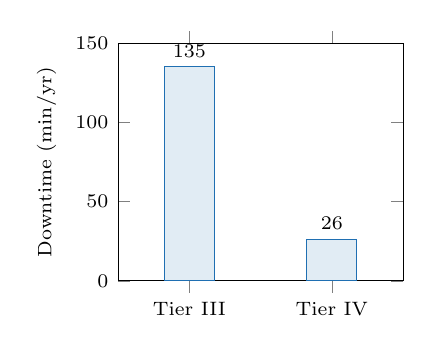
\begin{tikzpicture}
        \begin{axis}[
            ybar, width=5.2cm, height=4.6cm,
            ymin=0, ymax=150,
            ylabel={Downtime (min/yr)},
            symbolic x coords={Tier III, Tier IV},
            xtick=data, bar width=18pt,
            nodes near coords, nodes near coords style={font=\scriptsize},
            enlarge x limits=0.5,
            tick label style={font=\scriptsize},
            label style={font=\scriptsize},
          ]
          \addplot[fill=surf2, draw=accent] coordinates {(Tier III,135) (Tier IV,26)};
        \end{axis}
      \end{tikzpicture}
  \end{columns}
\end{frame}

\begin{frame}{Caveats}
  \begin{itemize}
    \item \textbf{Illustrative values.} Per-unit figures are industry-typical, not site-measured;
          swap in real MTBF/MTTR before use.
    \item \textbf{Human error \& common-cause failures dominate} real outages --- calculated
          availability is optimistic versus observed.
    \item \textbf{Define ``down'' explicitly.} Total loss vs.\ partial capacity vs.\ SLA breach;
          dual-corded (A/B) IT loads complicate single-path loss.
    \item \textbf{Infrastructure $\neq$ IT service availability.} State which layer is measured.
    \item \textbf{Planned maintenance excluded} --- the point of concurrent maintainability (Tier III+).
  \end{itemize}
\end{frame}

\begin{frame}[standout]{Takeaways}
  \begin{itemize}
    \item $A = \dfrac{\mathrm{MTBF}}{\mathrm{MTBF}+\mathrm{MTTR}}$; build up from an RBD.
    \item Series multiplies (lowers); parallel/redundancy squares unavailability (raises).
    \item Tier III $\approx$ 99.974\,\% $\,\to\,$ Tier IV $\approx$ 99.995\,\%: $\approx 5\times$ less downtime.
    \item The weakest non-redundant link sets the ceiling.
  \end{itemize}
\end{frame}

\end{document}
